\subsection{Test Methods}
There are a number of different types of tests appropriate for our project. The tests mentioned in this chapter are general tests that works equally well related to software development and hardware development. In Fig. \ref{fig:testing} a setup on how testing can be divided in to groups is displayed.

\begin{figure}[h]
    \centering
        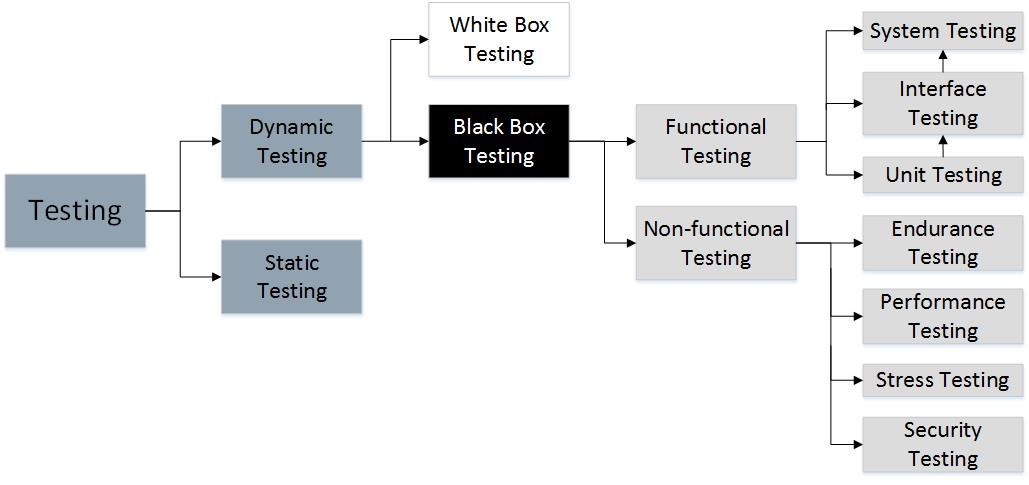
\includegraphics[width=0.9\textwidth]{VAPIQ-PICTURES/testing}
        \caption{Test Methods Diagram}
        \label{fig:testing}
\end{figure}

\subsubsection*{Static Testing}
The primary purpose of Static Testing or Static Verification is to find errors in documentation and code. We do this through review, analysis, inspection, and walk-through. The purpose of this is to find deviations from the stakeholder needs. The results can be used to optimize development processes and provide input to dynamic testing \cite{ref3}. 

\subsubsection*{Dynamic Testing}
Dynamic Testing can be conducted on the actual product. The purpose of this is to find deviations from expected values or the confirmed values \cite{ref3}. The main purpose of Dynamic Testing is to ensure consistency of the system.
\newpage

 